\documentclass{standalone}
\usepackage{amsmath,amssymb}
\usepackage{newtxtext,newtxmath}
\usepackage{xcolor}
\usepackage{tikz}
\usetikzlibrary{arrows.meta,positioning,calc,decorations.pathreplacing}

\definecolor{ink}{HTML}{1B1F23}
\definecolor{slate}{HTML}{555E68}
\definecolor{muted}{HTML}{8E96A0}
\definecolor{light}{HTML}{C6CCD2}
\definecolor{faint}{HTML}{E6E9ED}
\definecolor{quantum}{HTML}{2C5E8A}
\definecolor{quantumlight}{HTML}{6C9AC3}
\definecolor{quantumpale}{HTML}{DCE7F2}
\definecolor{ochre}{HTML}{B86B19}
\definecolor{ochrelight}{HTML}{E2B98B}
\definecolor{ochrepale}{HTML}{F6E9D8}

\newcommand{\pfmain}[1]{{\fontsize{7.6}{8.8}\selectfont\color{ink}#1}}
\newcommand{\pfsub}[1]{{\fontsize{7.0}{8.2}\selectfont\color{ink}#1}}
\newcommand{\pfslate}[1]{{\fontsize{7.0}{8.2}\selectfont\color{slate}#1}}
\newcommand{\pfquantum}[1]{{\fontsize{7.0}{8.2}\selectfont\color{quantum}#1}}
\newcommand{\pfochre}[1]{{\fontsize{7.0}{8.2}\selectfont\color{ochre}#1}}

\newcommand{\haty}{%
  \tikz[baseline=(Y.base)]{%
    \node[inner sep=0pt, outer sep=0pt] (Y) {$y$};
    \draw[line width=0.45pt, line cap=round, line join=round]
      ([xshift=0.3pt,yshift=1.25pt]Y.north west) -- ([yshift=2.45pt]Y.north) -- ([xshift=-0.3pt,yshift=1.25pt]Y.north east);
  }%
}

\tikzset{
  pfarrow/.style={-{Stealth[length=3.3pt, width=2.4pt]}, line width=0.65pt, draw=ink},
  pfmutedarrow/.style={-{Stealth[length=3.2pt, width=2.3pt]}, line width=0.60pt, draw=slate},
  pfqgate/.style={
    rectangle, draw=ink, fill=white, line width=0.65pt,
    minimum height=0.225in, inner sep=2.2pt,
    font=\fontsize{7.0}{8.0}\selectfont, text=ink
  }
}

\begin{document}
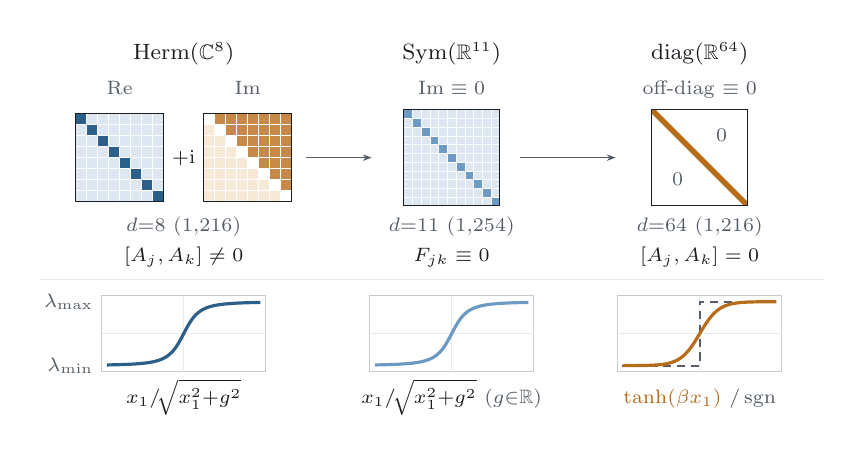
\begin{tikzpicture}[x=1in, y=1in]
  \useasboundingbox (0,-0.05in) rectangle (4.0448in, 1.93in);
  \fill[white] (0,-0.05) rectangle (4.0448, 1.93);

  % Equal-capacity operator-swap ladder: Herm(C^8) -> Sym(R^11) -> diag(R^64)
  \node[anchor=base, inner sep=0pt] at (0.78, 1.77) {\pfmain{$\mathrm{Herm}(\mathbb{C}^8)$}};
  \node[anchor=base, inner sep=0pt] at (0.46, 1.595) {\pfslate{$\mathrm{Re}$}};
  \node[anchor=base, inner sep=0pt] at (1.10, 1.595) {\pfslate{$\mathrm{Im}$}};

  \foreach \r in {0,...,7} {
    \foreach \c in {0,...,7} {
      \pgfmathsetmacro{\xz}{0.24 + \c*0.055}
      \pgfmathsetmacro{\yz}{1.50 - (\r+1)*0.055}
      \ifnum\r=\c
        \fill[quantum] (\xz, \yz) rectangle ++(0.055, 0.055);
      \else
        \fill[quantumpale] (\xz, \yz) rectangle ++(0.055, 0.055);
      \fi
      \draw[white, line width=0.20pt] (\xz, \yz) rectangle ++(0.055, 0.055);
    }
  }
  \draw[ink, line width=0.55pt] (0.24, 1.06) rectangle (0.68, 1.50);

  \node[anchor=center, inner sep=0pt] at (0.78, 1.28) {\pfsub{$+\mathrm{i}$}};

  \foreach \r in {0,...,7} {
    \foreach \c in {0,...,7} {
      \pgfmathsetmacro{\xz}{0.88 + \c*0.055}
      \pgfmathsetmacro{\yz}{1.50 - (\r+1)*0.055}
      \ifnum\r=\c
        \fill[white] (\xz, \yz) rectangle ++(0.055, 0.055);
      \else
        \ifnum\r<\c
          \fill[ochre!80] (\xz, \yz) rectangle ++(0.055, 0.055);
        \else
          \fill[ochrepale] (\xz, \yz) rectangle ++(0.055, 0.055);
        \fi
      \fi
      \draw[white, line width=0.20pt] (\xz, \yz) rectangle ++(0.055, 0.055);
    }
  }
  \draw[ink, line width=0.55pt] (0.88, 1.06) rectangle (1.32, 1.50);

  \node[anchor=base, inner sep=0pt] at (0.78, 0.91) {\pfslate{$d{=}8$ ($1{,}216$)}};
  \node[anchor=base, inner sep=0pt] at (0.78, 0.76) {\pfsub{$[A_j,A_k]\neq 0$}};

  \draw[pfmutedarrow] (1.39, 1.28) -- (1.72, 1.28);

  \node[anchor=base, inner sep=0pt] at (2.12, 1.77) {\pfmain{$\mathrm{Sym}(\mathbb{R}^{11})$}};
  \node[anchor=base, inner sep=0pt] at (2.12, 1.595) {\pfslate{$\mathrm{Im}\equiv 0$}};

  \foreach \r in {0,...,10} {
    \foreach \c in {0,...,10} {
      \pgfmathsetmacro{\xz}{1.88 + \c*0.043636}
      \pgfmathsetmacro{\yz}{1.52 - (\r+1)*0.043636}
      \ifnum\r=\c
        \fill[quantumlight] (\xz, \yz) rectangle ++(0.043636, 0.043636);
      \else
        \fill[quantumpale] (\xz, \yz) rectangle ++(0.043636, 0.043636);
      \fi
      \draw[white, line width=0.16pt] (\xz, \yz) rectangle ++(0.043636, 0.043636);
    }
  }
  \draw[ink, line width=0.55pt] (1.88, 1.04) rectangle (2.36, 1.52);

  \node[anchor=base, inner sep=0pt] at (2.12, 0.91) {\pfslate{$d{=}11$ ($1{,}254$)}};
  \node[anchor=base, inner sep=0pt] at (2.12, 0.76) {\pfsub{$F_{jk}\equiv 0$}};

  \draw[pfmutedarrow] (2.46, 1.28) -- (2.94, 1.28);

  \node[anchor=base, inner sep=0pt] at (3.36, 1.77) {\pfmain{$\operatorname{diag}(\mathbb{R}^{64})$}};
  \node[anchor=base, inner sep=0pt] at (3.36, 1.595) {\pfslate{off-diag $\equiv 0$}};

  \fill[white] (3.12, 1.04) rectangle (3.60, 1.52);
  \begin{scope}
    \clip (3.12, 1.04) rectangle (3.60, 1.52);
    \draw[ochre, line width=2.0pt] (3.12, 1.52) -- (3.60, 1.04);
  \end{scope}
  \draw[ink, line width=0.55pt] (3.12, 1.04) rectangle (3.60, 1.52);
  \node[anchor=center, inner sep=0pt] at (3.47, 1.39) {\pfslate{$0$}};
  \node[anchor=center, inner sep=0pt] at (3.25, 1.17) {\pfslate{$0$}};

  \node[anchor=base, inner sep=0pt] at (3.36, 0.91) {\pfslate{$d{=}64$ ($1{,}216$)}};
  \node[anchor=base, inner sep=0pt] at (3.36, 0.76) {\pfsub{$[A_j,A_k]=0$}};

  % Exact 1D readout slices y_hat(x_1): avoided crossing vs Gibbs tanh(beta x_1) vs Voronoi sgn(x_1)
  \draw[faint, line width=0.55pt] (0.06, 0.67) -- (3.98, 0.67);
  \node[anchor=east, inner sep=0pt] at (0.33, 0.56) {\pfslate{$\lambda_{\max}$}};
  \node[anchor=east, inner sep=0pt] at (0.33, 0.24) {\pfslate{$\lambda_{\min}$}};

  \draw[light, line width=0.45pt] (0.37, 0.21) rectangle (1.19, 0.59);
  \draw[faint, line width=0.40pt] (0.78, 0.21) -- (0.78, 0.59);
  \draw[faint, line width=0.40pt] (0.37, 0.40) -- (1.19, 0.40);
  \draw[quantum, line width=1.15pt, smooth, samples=55, domain=-3:3]
    plot ({0.78 + 0.128*\x}, {0.40 + 0.160*(\x / sqrt(\x*\x + 0.4225))});
  \node[anchor=base, inner sep=0pt] at (0.78, 0.05)
    {\pfsub{$x_1/\!\sqrt{x_1^2{+}g^2}$}};

  \draw[light, line width=0.45pt] (1.71, 0.21) rectangle (2.53, 0.59);
  \draw[faint, line width=0.40pt] (2.12, 0.21) -- (2.12, 0.59);
  \draw[faint, line width=0.40pt] (1.71, 0.40) -- (2.53, 0.40);
  \draw[quantumlight, line width=1.15pt, smooth, samples=55, domain=-3:3]
    plot ({2.12 + 0.128*\x}, {0.40 + 0.160*(\x / sqrt(\x*\x + 0.4225))});
  \node[anchor=base, inner sep=0pt] at (2.12, 0.05)
    {\pfsub{$x_1/\!\sqrt{x_1^2{+}g^2}$}\;\pfslate{($g{\in}\mathbb{R}$)}};

  \draw[light, line width=0.45pt] (2.95, 0.21) rectangle (3.77, 0.59);
  \draw[faint, line width=0.40pt] (3.36, 0.21) -- (3.36, 0.59);
  \draw[faint, line width=0.40pt] (2.95, 0.40) -- (3.77, 0.40);
  \draw[slate, line width=0.80pt, densely dashed]
    (2.97, 0.24) -- (3.36, 0.24) -- (3.36, 0.56) -- (3.75, 0.56);
  \draw[ochre, line width=1.15pt, smooth, samples=55, domain=-3:3]
    plot ({3.36 + 0.128*\x}, {0.40 + 0.160*((exp(2.676*\x) - 1)/(exp(2.676*\x) + 1))});
  \node[anchor=base, inner sep=0pt] at (3.36, 0.05)
    {\pfochre{$\tanh(\beta x_1)$}\;\pfslate{/\,$\operatorname{sgn}$}};
\end{tikzpicture}
\end{document}
